\subsection{Decentralized control}

In this section we will investigate the control of the four-tank process with a decentralized control. 

\paragraph{Minimum phase system}

In the minimum phase system the input $u_1$ is coupled with $y_1$ and $u_2$ is coupled with $y_2$. 

We will therefore use:

$$F_m(s) = \left[\begin{array}{cc} f_1(s) & 0 \\ 0 & f_2(s) \end{array}\right]$$

\paragraph{Non-minimum phase system}

In the non-minimum phase system the input $u_1$ is coupled with $y_2$ and $u_2$ is coupled with $y_1$. 

We will therefore use:

$$F_{nm}(s) = \left[\begin{array}{cc} 0 & f_1(s) \\ f_2(s) & 0 \end{array}\right]$$

\subsubsection{Exercice}

The specification of the controlled system are the following:

\begin{shortitemize}
    \item Phase margin: $\varphi_m = \pi/3$
    \item Crossover frequency: 
        \begin{shortitemize}
            \item Minimum phase system: $\omega_{c,m} = .1$rad/s
            \item Non-minimum phase system: $\omega_{c,nm} = .02$rad/s
        \end{shortitemize}
\end{shortitemize}

As we can see $\omega_{c,nm} \leq .029$ (see Exercise 3.1.2). Therefore the RHP zero will not be a problem.

The controller are designed using the method depicted in the subject. 
We have the following values:

\begin{center}
    \begin{tabular}{|c|cc|}
        \hline
        & $f_1(s)$ & $f_2(s)$ \\
        \hline
        $F_{m}(s)$ & & \\
        $F_{nm}(s)$ & & \\
       \hline 
    \end{tabular}
\end{center}


\subsubsection{Exercise}
\paragraph{Minimum phase model}

Figure \ref{singm} shows the maximum and minimum singular value of $S$ and $T$ as a function of the frequency. 
In this minimum-phase case, no restricting criteria was formulated regarding to $S$ and $T$.

\begin{figure}[h!t]
    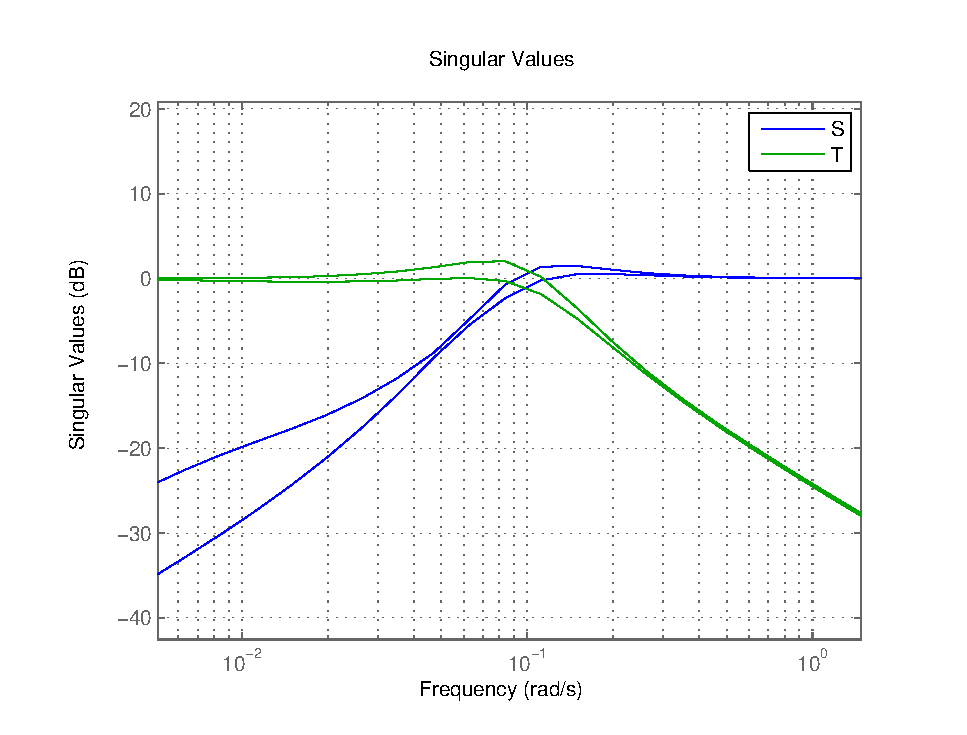
\includegraphics[width=\columnwidth]{fig/ST322m.eps}
    \caption{Singular values of $S$ and $T$ for the minimum phase system}
    \label{singm}
\end{figure}

\paragraph{Non-minimum phase model}


Figure \ref{singnm} shows the maximum and minimum singular value of $S$ and $T$ as a function of the frequency. 
In this non-minimum-phase case, since there is a RHP zero in the transfer matrix we had the following criteria regarding the bandwith limitation : $\omega_{BS} \leq 0.029$. This criteria is fulfilled.


\begin{figure}[h!t]
    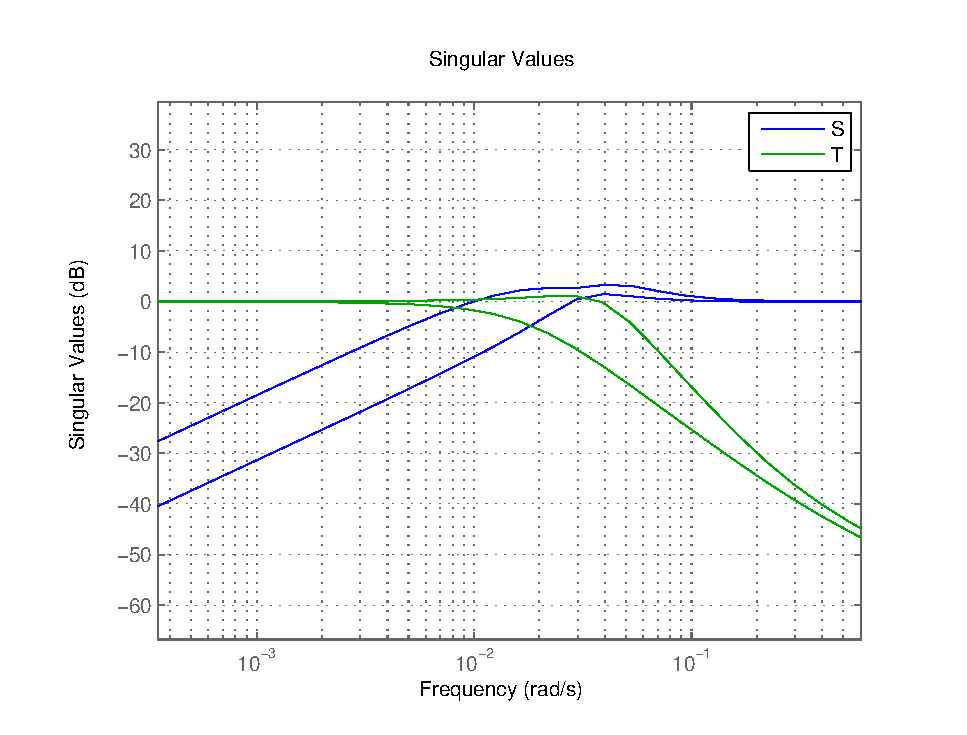
\includegraphics[width=\columnwidth]{fig/ST322nm.eps}
    \caption{Singular values of $S$ and $T$ for the non-minimum phase system}
    \label{singnm}
\end{figure}


\subsubsection{Exercise}

Using simulink we simulate the closed-loop system for an input:
$$ r(t) = \left\{\begin{array}{rcl} r_1(t) & = & u_{t\geq 100} \\ r_2(t) & = & u_{t\geq 500} \end{array}\right.$$

\paragraph{Minimum phase model}

Figure \ref{simum} shows the output $y_1$ and $y_2$ of the closed-loop system in the minimum phase case. 
The control quality is the following: 
\begin{center}
\begin{tabular}{|c|ccc|}
    \hline
    & Overshoot& Overshoot& Rise\\ 
    & coupled & non-coupled & time \\
    \hline
    $y_1$ & $12\%$ & $0.1$ & $30$s  \\
    $y_2$ & $13\%$ & $0.1$ & $30$s  \\
    \hline
\end{tabular}
\end{center}

\begin{figure}[h!t]
    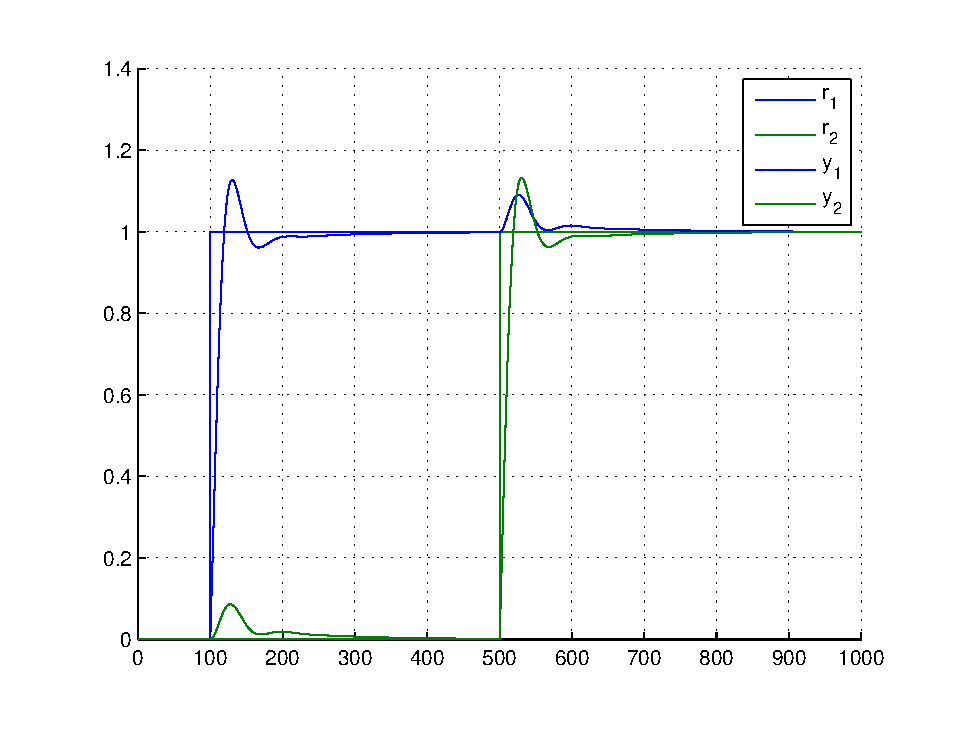
\includegraphics[width=\columnwidth]{fig/controlledouputm.eps}
    \caption{Response of the minimum phase system to $r(t)$}
    \label{simum}
\end{figure}

\paragraph{Non-minimum phase model}

Figure \ref{simunm} shows the output $y_1$ and $y_2$ of the closed-loop system in the non-minimum phase case. 
The control quality is the following: 
\begin{center}
\begin{tabular}{|c|ccc|}
    \hline
    & Overshoot& Overshoot& Rise\\ 
    & coupled & non-coupled & time \\
    \hline
    $y_1$ & $0\%$ & $0.5$ & $350$s  \\
    $y_2$ & $0\%$ & $0.35$ & $200$s  \\
    \hline
\end{tabular}
\end{center}

\begin{figure}[h!t]
    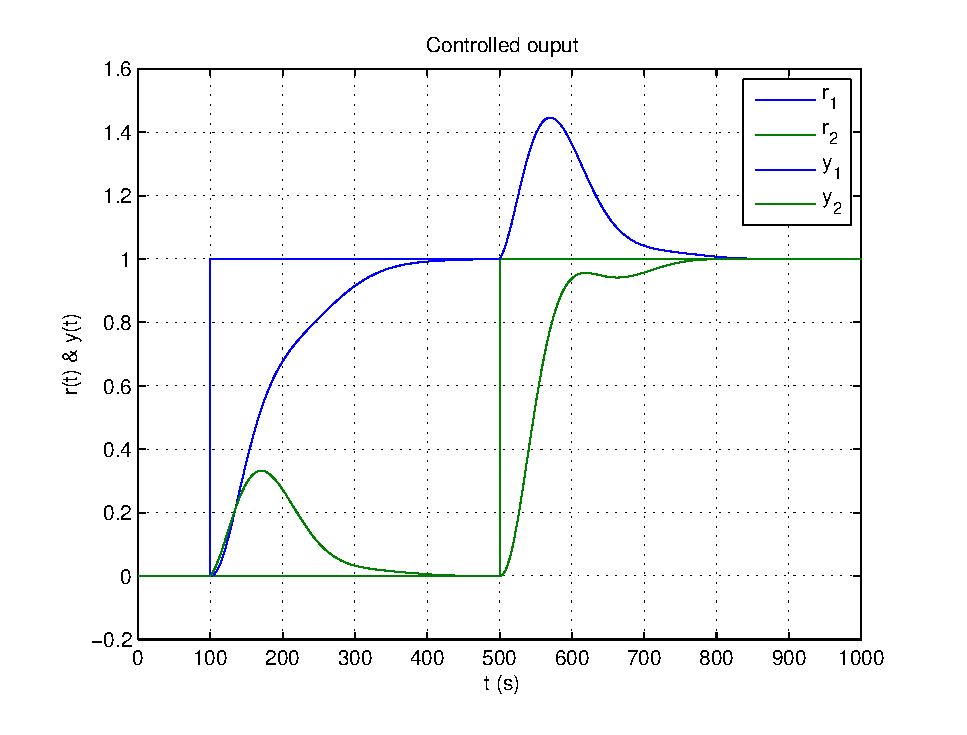
\includegraphics[width=\columnwidth]{fig/controlledouputnm.eps}
    \caption{Response of the non-minimum phase system to $r(t)$}
    \label{simunm}
\end{figure}

\paragraph{Results}

Figure \ref{simum} \& \ref{simunm} shows that the outputs are indeed coupled. 
However the control performance are more satisfying in the minimum-phase case. This is legit since the minimum-phase system do not present a RHP zero.

\subsubsection{Exercise}

As we have seen in the previous exercise, the control performance are better in the minimum phase case. 
(Even if its a bad idea in most cases to implement a decentralized controller).
Moreover since the non-minimum phase system presents a zero in the RHP it is more complicated to design this kind of controller 

